The assumption is made that the grid is fine grained and corresponds to a surface on earth. Each cell in the grid has a boolean and 

    $grid[x][y] == true$ for $x,y\in [0;\text{WORLD\_SIZE}]$
    
would represent a surface with lossless internet connection on every point. Each balloon occupies exactly one point in the grid but supplies coverage to the neighbouring area. The size of that area is controlled by the parameter RANGE. This is better displayed in figure \ref{fig:gridAssupmtions}.
\begin{figure}[H]
    \centering
    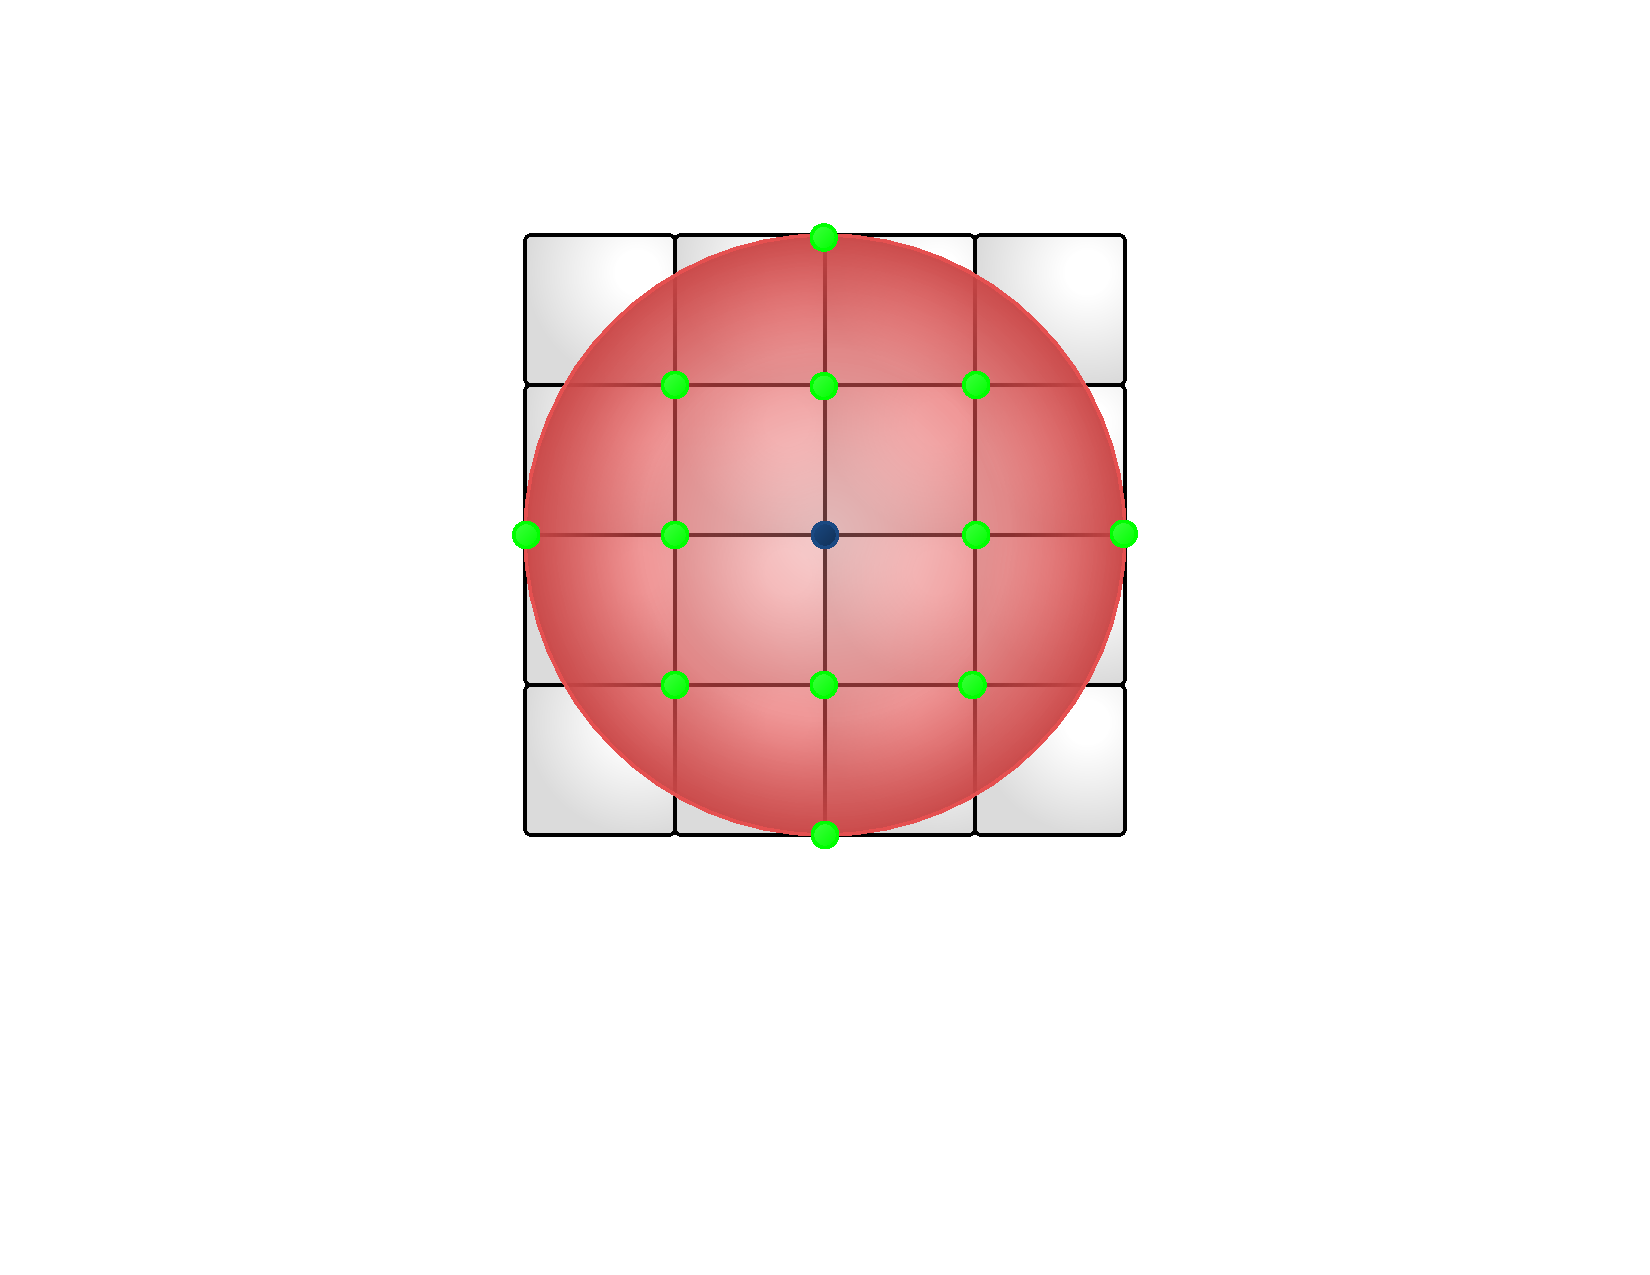
\includegraphics[width=\textwidth, trim=4cm 6cm 4cm 3cm, clip]{graphics/coverage.pdf}
    \caption{The figure displays the coverage in a 5x5 grid with a balloon at (2,2) and RANGE=2}
    \label{fig:gridAssupmtions}
\end{figure}
The actual placement of each balloon in regards to coverage on earth is somewhat irrelevant for this model, since the goal is to distribute the balloons evenly and keep them moving in an organized fashion, i.e keep each cell in grid above and close to 1. The grid of balloons is an abstract measurement of the distribution of the balloons and is sufficiently good tool to measure the quality of any control algorithm. 

The movement of a balloon in a grid is similar to the old Nintendo games. 

\begin{figure}[H]
    \centering
    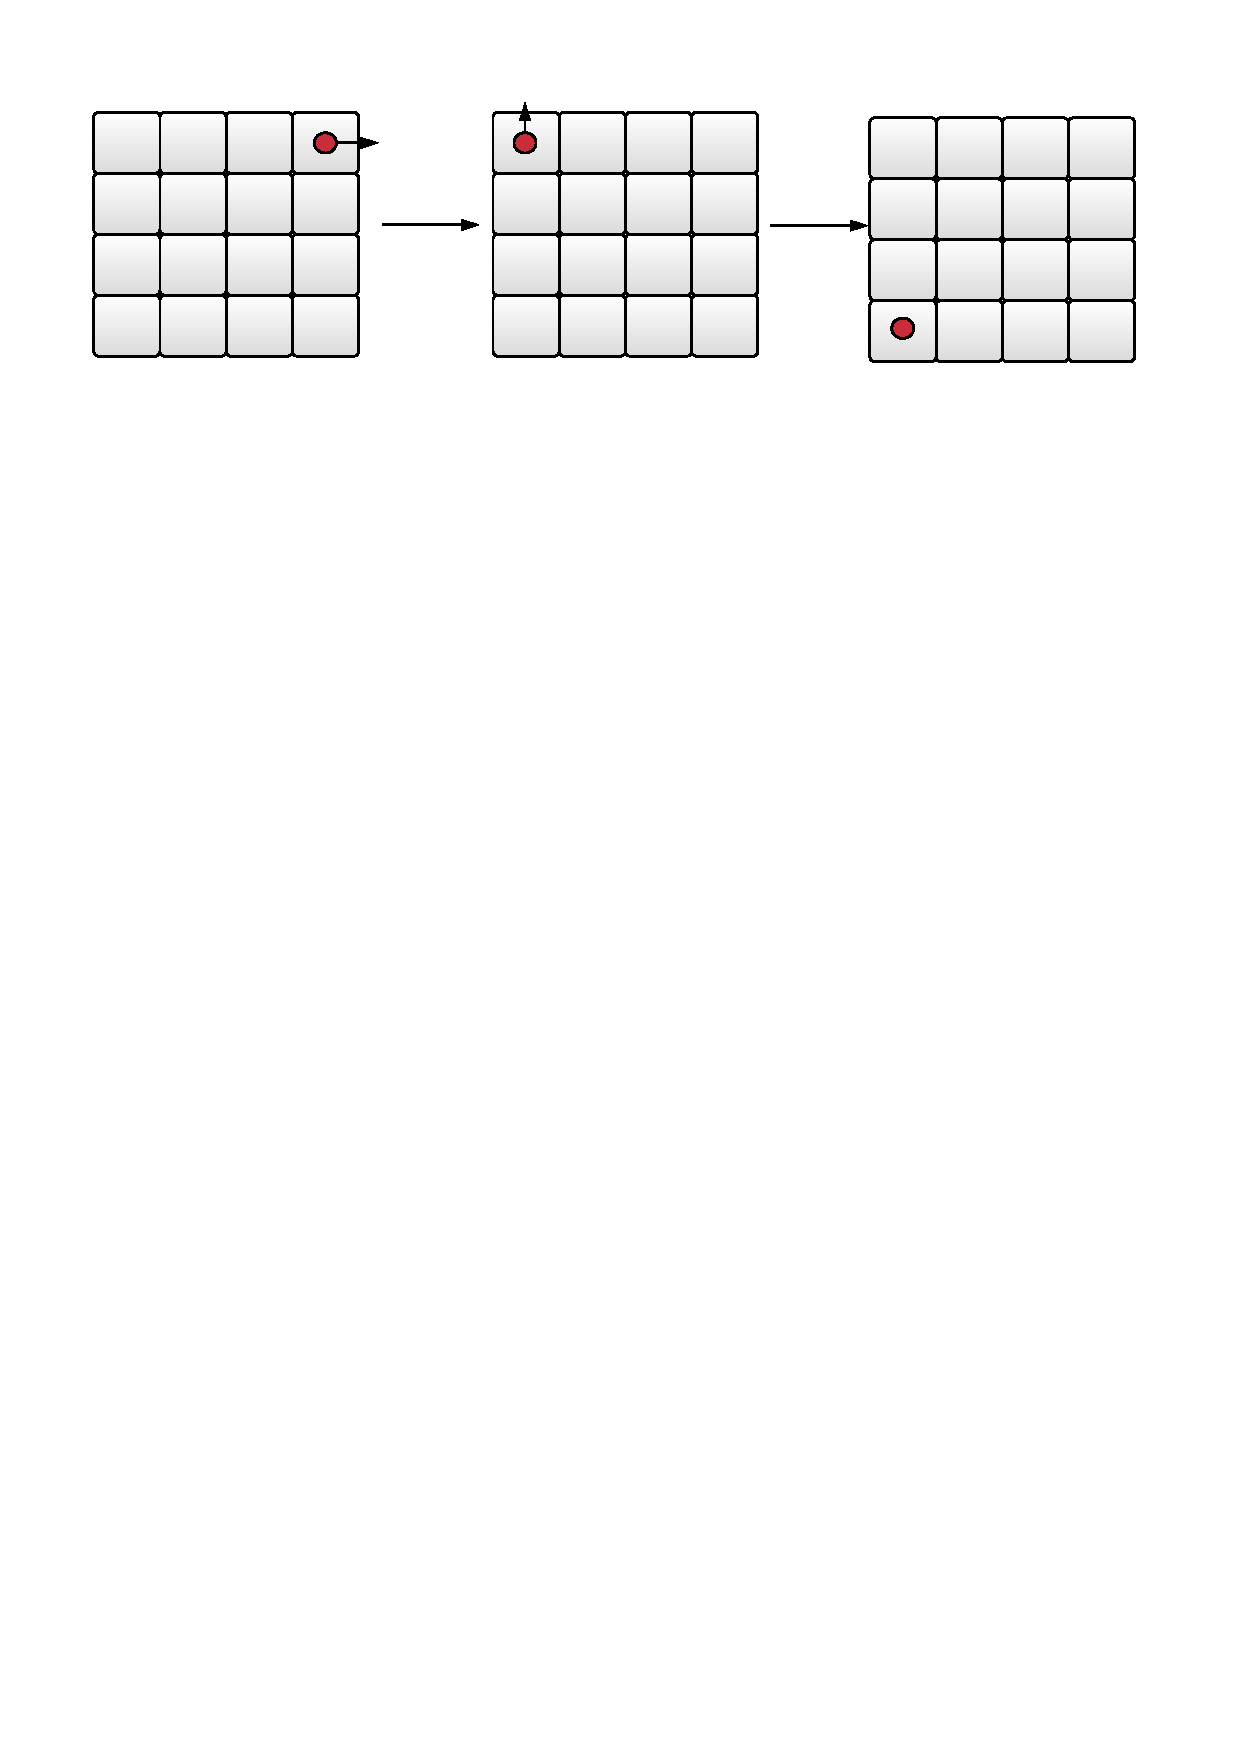
\includegraphics[width=\textwidth, trim=1cm 22cm 1cm 1cm, clip]{graphics/borderBehaviour.pdf}
    \caption{Border Behaviour}
    \label{fig:bb}
\end{figure}

When a balloon exits the grid it appears on the opposite site. This is done as a rudimentary attempt to resemble the behaviour of an object in a spherical grid when flattened out. 

In the model the balloons are a point in a grid, without a mass or volume. Also, the balloons do not move to a different spot in a continuous motion but are teleported between places. Removed from point A, and spawned at a point B. Multiple balloons are allowed to occupy the same space without any conflicts or implications. This is a simplification of the real life problem, but does not have to be included in the model as the odds of a crash are trivial when the size of the space the balloons occupy are taken into consideration. The model is however constructed so that removing this assumption would be easy. With the \textit{removeBalloon()} function the implication of a crash is easily implemented.

The current lifetime of a balloon is a fixed number in this model, which is an unlikely event in the real life problem. The balloons can however still not hover forever so this model parameter was necessary. The balloon is removed from the grid at the point where it was located when it reached is maximum age. This is convenient when modelling, but maybe not in the real life problem, since the balloon could be hovering over the sea, or a city, when it reaches its limit. The assumption is made that the balloon can be safely landed at every point in the grid. 

All new balloons are launched from the same place, at cell (0,0) in the grid. More launching places could easily be implemented by modifying the createBalloon() function or by using the override function createBalloon(int x, int y) which lets the user choose a specific location to which the new instance of the Balloon class should be created.

The weather data and the vertical movement of the balloons has been simplified greatly. The mock data created has been created really conveniently to give the balloons as many directions to choose from as possible. This is not always the case in the stratosphere. Furthermore, the division between different wind layers is not as clear as portrayed in this model. The data is however realistic enough to give weight to the model and display a lifelike behaviour of the balloons to some extent. The balloons move between two points in every step of the simulation, whether it is with one layer or another, and that behaviour is sufficient at this stage.

The assumption is made that the coverage on earth does not depend on the altitude of a balloon. This is a simplification since the signal strength from a balloon differs from altitude to altitude. This is overlooked in this model but can easily be implemented in an updated version, since this is only a matter of calculations and usage of units and measurements that already are available in this model. 


